\section{Determinants and Trace}

  The definition of the determinant is given first and then shown that it has the corresponding properties. We will work backward and construct the determinant from its properties. 

  \begin{definition}[Determinant]
    The determinant of a $n \times n$ matrix $A$, with column vectors $a_1, a_2, \cdots, a_n$, is a function
    \begin{equation}
      \det: \text{Mat}(n, \mathbb{F}) \longrightarrow \mathbb{F}
    \end{equation}
    with the following three properties
    \begin{enumerate}
      \item The determinant of the identity matrix is 1. 
      \begin{equation}
        \det{(I)} \equiv \det{(e_1, e_2, \cdots, e_n)} = 1
      \end{equation}
      \item Interchanging two columns $a_i$ and $a_j$ of $A$ once changes the sign of $\det{A}$. 
      \begin{equation}
        \det{(a_1, \cdots, a_i, \cdots, a_j, \cdots, a_n)} = -\det{(a_1, \cdots, a_j, \cdots, a_i, \cdots, a_n)}
      \end{equation}
      \item It is a multilinear function of the $n$ column vectors. 
      \begin{equation}
        \det{(a_1, \cdots, \lambda a_i + \mu a_i^\prime, \cdots a_n)} = \lambda \det{(a_1, \cdots, a_i, \cdots a_n)} + \mu \det{(a_1, \cdots, a_i^\prime, \cdots a_n)}
      \end{equation}
    \end{enumerate}
  \end{definition}

  \begin{figure}[H]
    \centering 
    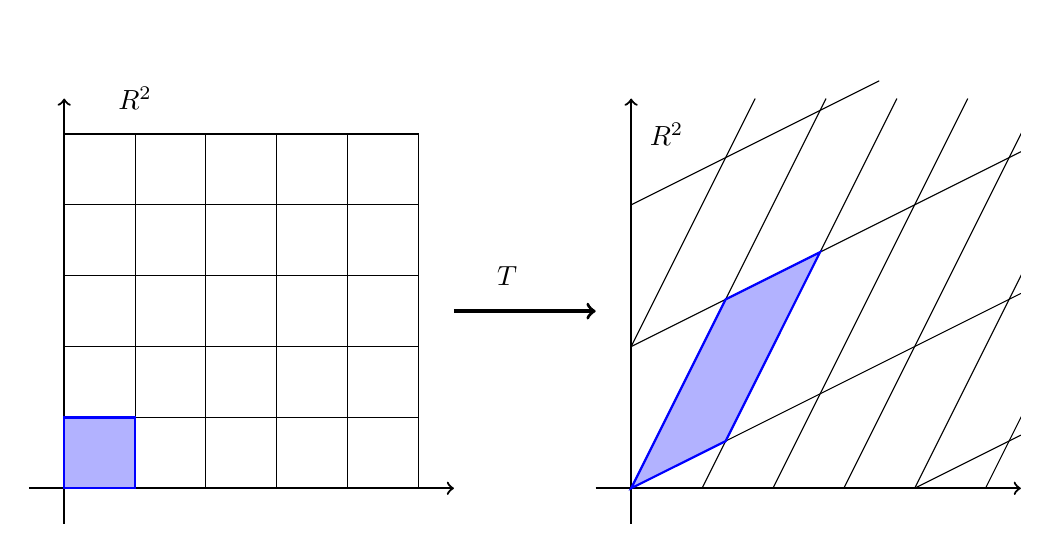
\begin{tikzpicture}[scale=0.9]
      % Left grid (domain)
      \begin{scope}[shift={(-5,0)}]
        % Draw grid
        \draw[step=1cm, black] (0,0) grid (5,5);
        
        % Draw axes
        \draw[thick, ->] (-0.5,0) -- (5.5,0);
        \draw[thick, ->] (0,-0.5) -- (0,5.5);
        
        % Label the space
        \node at (1,5.5) {$\mathbb{R}^2$};
        \fill[blue, opacity=0.3] (0,0) -- (1, 0) -- (1, 1) -- (0, 1) -- cycle;
        \draw[blue, thick] (0,0) -- (1, 0) -- (1, 1) -- (0, 1) -- cycle;

      \end{scope}
      
      % Transformation arrow
      \draw[->, very thick] (0.5,2.5) -- (2.5,2.5);
      \node at (1.25,3) {$T$};
      
      % Right grid (codomain)
      \begin{scope}[shift={(3,0)}]
        % Draw only axes
        \draw[thick, ->] (-0.5,0) -- (5.5,0);
        \draw[thick, ->] (0,-0.5) -- (0,5.5);
        
        % Label the space
        \node at (0.5,5) {$\mathbb{R}^2$};
        
        % Clip all drawing to stay within visible area
        \begin{scope}
          \clip (-0.5,-0.5) rectangle (5.5,6.5);
          
          % Existing lines with slope 1/2
          \draw[] (4,0) -- (5.5,0.75);
          \draw[] (0,0) -- (5.5,2.75);
          \draw[] (0,2) -- (5.5,4.75);
          \draw[] (0,4) -- (3.5,5.75);
          
          % New lines with slope 2
          \draw[] (5,0) -- (7.75,5.5);
          \draw[] (4,0) -- (6.75,5.5);
          \draw[] (3,0) -- (5.75,5.5);
          \draw[] (2,0) -- (4.75,5.5);
          \draw[] (1,0) -- (3.75,5.5); 
          \draw[] (0,0) -- (2.75,5.5); 
          \draw[] (0,2) -- (1.75,5.5); 
        \end{scope}
        \fill[blue, opacity=0.3] (0,0) -- (1.333,2.666) -- (2.666,3.333) -- (1.333,0.666) -- cycle;
        \draw[blue, thick] (0,0) -- (1.333,2.666) -- (2.666,3.333) -- (1.333,0.666) -- cycle;
      \end{scope}
    \end{tikzpicture}
    \caption{An important way to visualize determinants is by using the linear map visualization introduced before. That is, the determinant is the area of the transformed shaded unit square. } 
    \label{fig:determinant}
  \end{figure}

  \begin{theorem}
    The column vectors of $A$ are linearly dependent if and only if $\det{A} = 0$. 
  \end{theorem}
  \begin{proof}
    By linearity, it is sufficient to prove that if two column vectors $a_i$ and $a_j$ of a matrix $A$ are equal, then $\det{A} = 0$. This can be easily seen by property (ii) of determinants. 
  \end{proof}

  \begin{theorem}
    \begin{equation}
      \det{\bigg(\prod_i A_i \bigg)} = \prod_i \det{A_i}
    \end{equation}
  \end{theorem}

  \begin{theorem}
    A matrix is invertible if and only if its determinant is nonzero. 
  \end{theorem}
  \begin{proof}
    A matrix is invertible $\iff$ it is nonsingular $\iff$ its columns are linearly independent $\iff$ its determinant is nonzero, by the previous theorem. 
  \end{proof}

  \begin{corollary}
    Given $n \times n$ matrix $A$,
    \begin{equation}
      \det{(A^{-1})} = \frac{1}{\det{A}}
    \end{equation}
  \end{corollary}

  \begin{theorem}
    The determinants of similar matrices are equal. 
  \end{theorem}
  \begin{proof}
    Let $A$ and $B$ be similar matrices. Then, there exists an $S$ such that $A = S^{-1} B S$ and 
    \begin{equation}
      \det{(A)} = \det{(S^{-1} B S} = \det{(S^{-1})} \det{(B)} \det{(S)} = \det{B}
    \end{equation}
  \end{proof}

  This theorem implies that the determinant is an intrinsic property of a linear transformation, so it is invariant under a change of basis. That is, choosing different matrix representations of a linear transformation does not change the determinant.  

  \begin{corollary}
    \begin{equation}
      \det{(A)} = \det{(A^T)}
    \end{equation}
  \end{corollary}
  \begin{proof}
    $A$ is similar to $A^T$, which will be proven in chapter 6. 
  \end{proof}

  \begin{theorem}
    The properties of the determinant combined with the previous corollary implies that 
    \begin{enumerate}
      \item Adding a scalar multiple of a row/column to another row/column doesn't affect the determinant. 
      \item Interchanging two rows/columns switches the sign of the determinant. 
      \item Multiplying a row/column by $\alpha$ multiplies the determinant by $\alpha$. 
    \end{enumerate}
  \end{theorem}

  \begin{theorem}
    Let $A$ be an $n \times n$ matrix whose first column is $e_1$
    \begin{equation}
      A = \begin{pmatrix}
      1&*&*&* \\
      0 &&& \\
      \ldots& & A_{11}& \\
      0&&&
      \end{pmatrix}
    \end{equation}
    where $A_{11}$ is the $(n-1) \times (n-1)$ submatrix of $A$ with entries $a_{i j}, \; i, j > 1$. Given this, 
    \begin{equation}
      \det{A} = \det{A_{11}}
    \end{equation}
  \end{theorem}
  \begin{proof}
    Using column reduction, we can see that 
    \begin{equation}
      \det{A} = \det{\begin{pmatrix}
      1&0&0&0 \\
      0 &&& \\
      \ldots& & A_{11}& \\
      0&&&
      \end{pmatrix}}
    \end{equation}
    it is clear that the right hand side is equal to $\det{A_{11}}$ since it behaves exactly like $\det{A_{11}}$ with respect to the three properties. 
  \end{proof}

  \begin{corollary}
    Let $A$ be an upper or a lower triangular matrix. Then the determinant of $A$ is the product of its diagonal entries. That is,  
    \begin{equation}
      \det{A} = \prod_{i} a_{i i}
    \end{equation}
  \end{corollary}
  \begin{proof}
    We apply the previous theorem recursively to satisfy when $A$ is upper triangular. Since $\det{(A)} = \det{(A^T)}$, this fact can be applied to lower triangular matrices too. 
  \end{proof}

  It is once again verified that the three elementary row (and column) operations affect the determinant in the way stated in Theorem 5.5. To elaborate, since $E_1, E_2$, and $E_3$ are all lower triangular, we can compute their determinants easily
  \begin{align*}
    \det{E^1_{\alpha \times i + j}} = 1 \\
    \det{E^2_{i j}} = -1 \\
    \det{E^3_{\alpha \times i}} = \alpha
  \end{align*}
  and multiplying matrix $A$ by elementary matrices $E^1, E^2$, and $E^3$ multiplies the determinant by $1, -1$, and $\alpha$, respectively. 

  We can describe the determinant visually. Given a linear mapping $A: V \longrightarrow V$, we can fix any basis $\{e_1, e_2, \cdots, e_n\}$ on $V$. Note that these basis vectors do not need to be orthogonal, nor are they restricted to any magnitude. The set of vectors 
  \begin{equation}
    \Big\{ \sum_{i=1}^n c_i e_i \mid 0 \leq c_i \leq 1, i = 1, 2, \cdots, n\Big\}
  \end{equation}
  forms an $n$-dimensional parallelepiped in $V$. Let the volume of this parallelepiped be $U$. Let $W$ be the volume of the parallelepiped 
  \begin{equation}
    \Big\{ \sum_{i=1}^n c_i A e_i \mid 0<c_i<1, i = 1, 2, \cdots, n\Big\}
  \end{equation}
  which is formed by the transformed basis vectors $\{Ae_1, Ae_2, \cdots, Ae_n\}$. We can view this latter shape as the image of the first parallelepiped under transformation $A$. Then, 
  \begin{equation}
    \det{A} = W / V 
  \end{equation}
  That is, the ratio of the transformed parallelepiped to the original parallelepiped is the determinant. This is consistent with the properties of the determinant. For example, if $A$ is not isomorphic, then the parallelepiped will get "squished" into a lower-dimensional parallelepiped with volume $0$. The fact that we use a ratio between the original and transformed parallelepiped allows this value to be invariant under the basis that we use. 

  Computationally, finding the LUP decomposition of a matrix $A$ is the best known algorithm to compute the determinant of a general $n \times n$ matrix. That is, 
  \begin{equation}
    \det{A} = \det{L} \det{U} \det{P} = \pm \det{U} = \pm \prod_i u_{i i}
  \end{equation}
  since $\det{L} = 1$ and $\det{P} = \pm 1$. 

  There are other methods to compute the determinant. First, we state the simple but useful formula.

  \begin{theorem}
    \begin{equation}
      \det{\begin{pmatrix}
      a&b\\c&d 
      \end{pmatrix}} = a d - b c
    \end{equation}
  \end{theorem}

  \begin{definition}
    Given an $n \times n$ matrix $A$, the $(i j)$th minor of $A$, denoted $A_{i j}$, is the determinant of the $(n-1) \times (n-1)$ matrix formed by removing the $i$th row and $j$ th column from $A$. 
  \end{definition}

  \begin{theorem}[Laplace Expansion]
    Let $A$ be an $n \times n$ matrix and $j$ any index between $1$ and $n$. Then
    \begin{equation}
      \det{A} = \sum_i (-1)^{i + j} a_{i j} A_{i j}
    \end{equation}
    that is, the alternating sums of the $ij$th minors multiplied by the $ij$th entries in the $j$th column of $A$. This can be done by choosing an arbitrary $i$th row, which leads to the alternative formula 
    \begin{equation}
      \det{A} = \sum_j (-1)^{i + j} a_{i j} A_{i j} 
    \end{equation}
  \end{theorem}

  \begin{theorem}[Cramer's Rule]
    Given a system of linear equations in the form $A x = b$ where $A$ is an $n \times n$ matrix, the solutions of this system can be expressed with the formulas 
    \begin{equation}
      x_i = \frac{ \det{A_i}}{\det{A}}
    \end{equation}
    where $\det{A_i}$ is the matrix formed by replacing $a_i$, the $i$th column of $A$, by the column vector $b$. 
  \end{theorem}

  Albeit very computationally heavy, determinants can also be used to calculate the inverse of a matrix. 

  \begin{theorem}
    The inverse matrix $A^{-1}$ of an invertible matrix $A$ has the form 
    \begin{equation}
      (A^{-1})_{i j} = (-1)^{i+j} \frac{\det{A_{i j}}}{\det{A}}
    \end{equation}
  \end{theorem}

  \begin{definition}
    The trace of a square matrix $A$, denoted $\Tr{A}$, is the sum of its diagonal entries. 
    \begin{equation}
      \Tr(A) = \sum_{i} a_{ii}
    \end{equation}
  \end{definition}

  \begin{theorem}
    \begin{equation}
      \Tr(\lambda A + \alpha B) = \lambda \Tr(A) + \alpha \Tr(B)
    \end{equation}
  \end{theorem}
  \begin{proof}
    Obvious if we look at the entries of $A$ and $B$ and see that it is bilinear.
  \end{proof}

  \begin{theorem}[Cyclic Property of the Trace]
    \begin{equation}
      \Tr{\bigg(\prod_{i=1}^n A_i\bigg)} = \Tr{\bigg(A_n \prod_{i=1}^{n-1} A_i\bigg)}
    \end{equation}
  \end{theorem}
  \begin{proof}
    We first prove when $m=2$. Given that the subscripts $i j$ denote that $(i,j)$th element of a matrix, observe that
    \begin{align*}
      (AB)_{ij} = \sum_{k} A_{ik} B_{kj} & \implies (AB)_{ii} = \sum_{K} A_{ik} B_{ki} \\
      & \implies \Tr(AB) = \sum_{i} \sum_{k} A_{ik} B_{ki} \\
      & \;\;\;\;\;\;\;\;\;\;\;\;\;\;\;\;\;\;\;\;\;\;= \sum_{k} \sum_{i} B_{ki} B_{ik} = Tr(BA)
    \end{align*}
    Similarly, for $m=3$
    \begin{align*}
      (ABC)_{ij} = \sum_{k,l} A_{ik} B_{kl} C_{lj} \implies \Tr(ABC) & = \sum_{i,k,l} A_{ik} B_{kl} C_{li} \\ 
                                                                     & = \sum_{i,k,l} C_{li} A_{ik} B_{kl} = \Tr(CAB)
    \end{align*}
    And so we can generalize for $m$. 
  \end{proof}

  \begin{corollary}
    The trace is invariant under a change of basis. That is, the trace is an intrinsic property of a linear transformation since it does not change depending on how it is represented. 
  \end{corollary}
  \begin{proof}
    Given that $A$ is similar to $B$. 
    \begin{equation}
      \Tr(B) = \Tr(S A S^{-1}) = \Tr(S^{-1} S A) = \Tr(A) 
    \end{equation}
  \end{proof}

  \begin{theorem}
    Let $A$ be a $n \times n$ skew-symmetric matrix over $\mathbb{C}$ (or any field of characteristic $\neq 2$). If $n$ is odd, 
    \begin{equation}
      \det{A} = 0 
    \end{equation}
  \end{theorem}
  \begin{proof}
    \begin{equation}
      \det{A} = \det{A^T} = \det{-A} = (-1)^n \det{A} \implies \det{A} = 0 
    \end{equation}
  \end{proof}

  We can actually conclude something even futher about antisymmetric matrices. 

  \begin{theorem}
    The determinant of an antisymmetric matrix $A$ of even order is the square of a homogeneous polynomial of degree $n/2$ in the entries of $A$. That is, 
    \begin{equation}
      \det{A} = P^2
    \end{equation}
    The polynomial $P$ is called the \textbf{Pfaffian}. 
  \end{theorem}

  \begin{definition}
    A \textbf{Vandermonde matrix} is a square matrix whose columns form a geometric progression. That is, let $a_1, a_2, \cdots, a_n$ be $n$ scalars. Then, $V(a_1, a_2, \cdots, a_n)$ is the $n \times n$ matrix
    \begin{equation}
      \begin{pmatrix}
        1&1&\ldots&1&1 \\
        a_1&a_2&\ldots&a_{n-1}&a_n\\
        \vdots&\vdots&\ddots&\vdots&\vdots\\
        a_1^{n-2}&a_2^{n-2}&\ldots&a_{n-1}^{n-2}&a_n^{n-2}\\
        a_1^{n-1}&a_2^{n-1}&\ldots&a_{n-1}^{n-1}&a_n^{n-1}
      \end{pmatrix}
    \end{equation}
  \end{definition}

  \begin{theorem}
    The determinant of a Vandermonde matrix is
    \begin{equation}
      \det{V(a_1, a_2, \cdots, a_n)} = \prod_{j>i} (a_j - a_i)
    \end{equation}
  \end{theorem}

  A symmetry in the multivariable expression of a determinant can also reveal a symmetry in the matrix.

  \begin{example}[2019 Putnam A1]
    The symmetric polynomial 
    \begin{equation}
       f(x, y, z) = x^3 + y^3 + z^3 - 3 x y z
    \end{equation}
    can be expressed as the determinant of the $3 \times 3$ matrix
    \begin{equation}
      \det{\begin{pmatrix}
      x&y&z\\
      z&x&y\\
      y&z&x
      \end{pmatrix}}
    \end{equation}
  \end{example}

\subsection{Matrices in Block Form}

  \begin{theorem}
    Given $2 \times 2$ block matrices
    \begin{equation}
      X = \begin{pmatrix}
      A_1&B_1\\C_1&D_1
      \end{pmatrix}, \; \; Y = \begin{pmatrix}
      A_2&B_2\\C_2&D_2
      \end{pmatrix}
    \end{equation}
    We can compute $X Y$ similarly to regular matrix multiplication, treating the blocks as entries. 
    \begin{equation}
      X Y = \begin{pmatrix}
      A_1&B_1\\C_1&D_1
      \end{pmatrix} \begin{pmatrix}
      A_2&B_2\\C_2&D_2
      \end{pmatrix} = \begin{pmatrix}
      A_1 A_2 + B_1 C_2 & A_1 B_2 + B_1 D_2 \\
      C_1 A_2 + D_1 C_2 & C_1 B_2 + D_1 D_2 
      \end{pmatrix}
    \end{equation}
    Furthermore, this process can be done in general for any $m \times n$ block matrix $X$ and $n \times p$ block matrix $Y$. 
  \end{theorem}

  \begin{theorem}
    Given that $I_N, A, B$ are $n \times n$ matrices, define the $(2n) \times (2n)$ matrix 
    \begin{equation}
      X = \begin{pmatrix} I & 0 \\ A & B \end{pmatrix}
    \end{equation}
    Then 
    \begin{equation}
      \det{X} = \det{B}
    \end{equation}
  \end{theorem}
  \begin{proof}
    We can perform Gauss elimination to reduce $X$ without affecting the determinant.
    \begin{equation}
      \det{\begin{pmatrix} I&0\\A&B \end{pmatrix}} = \det{ \begin{pmatrix} I&0\\ 0&B \end{pmatrix}} = \det{B}
    \end{equation}
    since it satisfies the correct properties for $\det{B}$. 
  \end{proof}

  \begin{corollary}
    \begin{equation}
      \det{\begin{pmatrix} A&0\\C&D \end{pmatrix}} = \det{A} \det{D}
    \end{equation}
  \end{corollary}
  \begin{proof}
    \begin{equation}
      \det{\begin{pmatrix}
      A&0\\C&D 
      \end{pmatrix}} = \det{\begin{pmatrix}
      A&0\\C&I
      \end{pmatrix} \begin{pmatrix}
      I&0\\0&D
      \end{pmatrix}} = \det{\begin{pmatrix}
      A&0\\C&I
      \end{pmatrix}} \det{\begin{pmatrix}
      I&0\\0&D
      \end{pmatrix}}
    \end{equation}
  \end{proof}

  However, 
  \begin{equation}
    \det{\begin{pmatrix} A&B\\C&D \end{pmatrix}} \neq \det{A} \det{D} - \det{B} \det{C}
  \end{equation}

  Rather, we introduce the following theorem

  \begin{theorem}
    \begin{align}
      \det{\begin{pmatrix} A&B\\C&D \end{pmatrix}}  & = \det{(A)} \det{(D - C A^{-1} B)} \\
      & = \det{(D)} \det{(A - B D^{-1} C)}
    \end{align}
  \end{theorem}
  \begin{proof}
    \begin{equation}
      \begin{pmatrix} A&B\\C&D\end{pmatrix} = \begin{pmatrix}
      A&0\\C&I\end{pmatrix} \begin{pmatrix}
      I& A^{-1} B \\ 0 & D - C A^{-1} B
      \end{pmatrix}
    \end{equation}
    by similarity, equation $(6)$ is equal to equation $(7)$. 
  \end{proof}

  \begin{definition}[Block Diagonal Matrix]
    A \textbf{block diagonal matrix} is a square matrix in block form such that the diagonal blocks are square matrices and all off-diagonal blocks are zero matrices. 
    \begin{equation}
      A = \begin{pmatrix}
      A_1&0&\ldots&0\\
      0&A_2&\ldots&0\\
      \vdots&\vdots&\ddots&\vdots\\
      0&0&\ldots&A_k
      \end{pmatrix}
    \end{equation}
  \end{definition}

  \begin{theorem}
    Given a matrix $A$ in block diagonal form, with diagonal blocks $A_1, A_2, \cdots, A_k$,
    \begin{equation}
      \det{A} = \prod_{i=1}^k A_i, \; \; \Tr{A} = \sum_{i=1}^k \Tr{A_i}
    \end{equation}
    Furthermore, $A$ is invertible if and only if all the $A_i$'s are invertible, and 
    \begin{equation}
      A^{-1} = \begin{pmatrix}
      A_1&0&\ldots&0\\
      0&A_2&\ldots&0\\
      \vdots&\vdots&\ddots&\vdots\\
      0&0&\ldots&A_k
      \end{pmatrix} = \begin{pmatrix}
      A_1^{-1}&0&\ldots&0\\
      0&A_2^{-1}&\ldots&0\\
      \vdots&\vdots&\ddots&\vdots\\
      0&0&\ldots&A_k^{-1}
      \end{pmatrix}
    \end{equation}
  \end{theorem}
  \begin{proof}
    The results are obvious when performing block multiplication or Gauss Elimination. 
  \end{proof}

\subsection{Dodgson Condensation}

  We already know that the LUP decomposition is an algorithm used to compute the determinant of a general $n \times n$ matrix. We will introduce another, called \textbf{Dodgson condensation}. The algorithm can be described in the following steps.

  \begin{enumerate}
    \item Let $A$ be a given $n \times n$ matrix. Arrange $A$ so that no zeros occur in its interior (this can be done by any combination of elementary row or column operations that would not change the determinant). 
    \item Create an $(n-1) \times (n-1)$ matrix $B$ consisting of the determinants of every $2 \times 2$ submatrix of $A$. Explicitly, 
    \begin{equation}
      B = \det{\begin{pmatrix} a_{i,j} & a_{i,j+1} \\ a_{i+1,j} & a_{i+1,j+1} \end{pmatrix}}
    \end{equation}
    \item With this $(n-1) \times (n-1)$ matrix $B$, perform step $2$ to obtain an $(n-2) \times (n-2)$ matrix $C$. Divide each term in $C$ by the corresponding term in the interior of $A$. 
    \begin{equation}
      C_{i,j} = \det{\begin{pmatrix} b_{i,j} & b_{i,j+1} \\ b_{i+1,j} & b_{i+1,j+1} \end{pmatrix}} \bigg/ a_{i+1,j+1}
    \end{equation}
    \item Let $A = B$ and $B=C$. Repeat step $3$ as necessary until the $1 \times 1$ matrix is found, which is the determinant. 
  \end{enumerate}

  The reason that we do not want $0$s in $A$ is because then in doing step $3$ we may divide by $0$. 

  \begin{example}
    Let us find
    \begin{equation}
      \det{\begin{pmatrix}
      -2&-1&-1&-4\\-1&-2&-1&-6\\-1&-1&2&4\\2&1&-3&-8
      \end{pmatrix}}
    \end{equation}
    All of the interior elements are nonzero, so there is no need to rearrange the matrix. We calculate
    \begin{equation}
      \begin{pmatrix}
      -2&-1&-1&-4\\-1&-2&-1&-6\\-1&-1&2&4\\2&1&-3&-8
      \end{pmatrix} \rightarrow \begin{pmatrix}
      3&-1&2\\-1&-5&8\\1&1&-4
      \end{pmatrix} \rightarrow \begin{pmatrix}
      -16&2\\4&12
      \end{pmatrix}
    \end{equation}
    With this $2 \times 2$ matrix, we must divide each term by the interior of the original $A$. 
    \begin{equation}
      \begin{pmatrix}
      -16/-2 & 2/-1\\4/-1 & 12/2
      \end{pmatrix} = \begin{pmatrix}
      8&-2\\-4&6
      \end{pmatrix}
    \end{equation}
    Calculating this determinant gives $40$, and dividing by the interior of the $3 \times 3$ matrix $(-5)$ gives $\det{A} = 40/-5 = -8$. 
  \end{example}

\subsection{Matrix Calculus}

  There is nothing special about matrix calculus on its own, since matrices are themselves vectors; they can be sufficiently analyzed using vector calculus. Regardless, we will emphasize a few points. Let
  \begin{equation}
    A: \mathbb{R} \longrightarrow \text{Mat}(m \times n, \mathbb{R})
  \end{equation}
  be a matrix valued differential function. That is, the $m \times n$ component functions of $A$ is differentiable. Then, just like in calculus, we introduce differentiation rules.
  \begin{align*}
    & \frac{d}{d x} \big( A(t) + B(t)\big) = \frac{d}{d t} A(t) + \frac{d}{d t} B(t) \\
    & \frac{d}{d x} \big( c A(t)\big) = c \frac{d}{d t} A(t)
  \end{align*}
  The scalar multiplication can actually be extended. By linearity (of matrix multiplication), we can say that if $A$ is independent of $t$, then 
  \begin{equation}
    \frac{d}{d x} A B (x) = A \frac{d}{d x} B(x)
  \end{equation}
  The linearity of the derivative allows us to state more rules. Given that $v: \mathbb{R}^n \longrightarrow \mathbb{R}$ is a scalar valued function and $l \in (\mathbb{R}^n)^*$, then  
  \begin{equation}
    \frac{d}{d x} l \big( v(x) \big) = l \bigg( \frac{d}{d x} v(x) \bigg)
  \end{equation}
  This result can be extended to when $v$ is replaced by matrix valued function $A$ and $l$ is replaced by $\phi: \text{Mat}(m \times n, \mathbb{R}) \longrightarrow \mathbb{R}$. 
  \begin{equation}
    \frac{d}{d x} \phi \big( A(x) \big) = \phi \bigg( \frac{d}{d x} A(x) \bigg)
  \end{equation}
  Since the trace is a linear operator, we have the following theorem. 

  \begin{theorem}
    Given a linear function $A: \mathbb{R} \longrightarrow \text{Mat}(n, \mathbb{R})$ with paramater $x$, 
    \begin{equation}
      \frac{d}{d x} \Tr{A} = \Tr \bigg( \frac{d}{d x} A \bigg)
    \end{equation}
    Note that $A$ in here really means $A(x)$.
  \end{theorem}

  The product rule of matrix calculus is similar.
  \begin{equation}
    \frac{d}{d x} A B = \bigg(\frac{d}{d x} A\bigg) \cdot B + A \cdot \bigg(\frac{d}{d x} B \bigg)
  \end{equation}
  It is also noting that the derivative of the inner product of two vector valued functions $v, w: \mathbb{R} \longrightarrow \mathbb{R}^n$ is 
  \begin{equation}
    \frac{d}{d x} \big( v(x), w(x) \big) = \Big( \frac{d}{d x} v(x), w(x) \Big) + \Big( v(x), \frac{d}{d x} w(x) \Big)
  \end{equation}

  \begin{definition}
    A matrix valued function $A$ is \textbf{invertible at a point $x \in \mathbb{R}$} if there exists a function, denoted $A^{-1}$ such that
    \begin{equation}
      A(x) A^{-1} (x) = A^{-1}(x) A(x) = I
    \end{equation}
    where $I$ is the identity matrix. If there exists such $A^{-1}$ for all values $x \in \mathbb{R}$, then $A$ is said to be \textbf{invertible}. 
  \end{definition}

  \begin{theorem}
    Let $A$ be a matrix valued function, differentiable and invertible. Then, the function $A^{-1}$ is also differentiable and 
    \begin{equation}
      \frac{d}{d x} A^{-1} = - A^{-1} \bigg( \frac{d}{d x} A \bigg) A^{-1}
    \end{equation}
  \end{theorem}
  \begin{proof}
    We derive this using the product rule. 
    \begin{align*}
      0 = \frac{d}{d x} I & = \frac{d}{d x} \big( A(x) A^{-1} (x) \big) \\
      & = A(x) \bigg(\frac{d}{d x} A^{-1} (x) \bigg) + \bigg( \frac{d}{d x} A(x) \bigg) A^{-1} (x) \\
      \implies \frac{d}{d x} A^{-1} (x) & = - A^{-1} (x) \bigg( \frac{d}{d x} A(x) \bigg) A^{-1}(x)
    \end{align*}
  \end{proof}
  Note that the chain rule is a rule of differentiaion that applies for scalar valued functions. That is, given $f: V \longrightarrow \mathbb{R}$ and $g: \mathbb{R} \longrightarrow V$ ($V$ vector space), 
  \begin{equation}
    \frac{d}{d x} f \circ g (x) = f^\prime \big( g(x) \big) \cdot \frac{d}{d x} g(x)
  \end{equation}
  The $\cdot$ operation in the right hand side is the operation of multiplication in the field $\mathbb{R}$. But given $f: \text{Mat}(n, \mathbb{R}) \longrightarrow \mathbb{R}$ and $A \mathbb{R} \longrightarrow \text{Mat}(n, \mathbb{R})$, multiplication within the algebra of matrices are inherently different than component-wise operations, so the chain rule does not apply (it would apply if matrix multiplication was defined component-wise). 

  \begin{example}
    Let $f(A) \equiv A^2$, and let $A$ be a matrix valued function. Then, 
    \begin{align*}
      \frac{d}{d x} f \circ A(x) = \frac{d}{d x} \big( A(t) \big)^2 & = \bigg( \frac{d}{d x} A(x) \bigg) \cdot A(x) + A(x) \cdot \bigg( \frac{d}{d x} A(x) \bigg) \\
      & \neq 2 A(x) \cdot \frac{d}{d x} A(x)
    \end{align*}
    since matrix multiplication is in general not commutative. 
  \end{example}

  \begin{theorem}
    \begin{equation}
      \frac{d}{d x} A^k = A^\prime A^{k-1} + A A^\prime A^{k-2} + \cdots + A^{k-2} A^\prime A + A^{k-1} A^\prime
    \end{equation}
  \end{theorem}
  \begin{proof}
    We inductively apply the product rule
    \begin{equation}
      \frac{d}{d x} A^k = A^\prime A^{k-1} + A \frac{d}{d x} A^{k-1}
    \end{equation}
  \end{proof}

  \begin{corollary}
    Given any polynomial $p$ with $A$ a differentiable, square matrix valued function, if $A$ and $A^\prime$ commute, then 
    \begin{equation}
      \frac{d}{d x} p(A) = p^\prime (A) A^\prime
    \end{equation}
  \end{corollary}
  \begin{proof}
    We can completely define differentiation over the vector space of polynomials with the formula
    \begin{equation}
      \frac{d}{d x} A^k = k A^{k-1} A^\prime \; \forall k \in \mathbb{N}
    \end{equation}
  \end{proof}

  \begin{corollary}
    Given polynomial $p$ with $A$ a differentiable, square matrix valued function, 
    \begin{equation}
      \frac{d}{d x} \Tr{p(A)} = \Tr{\big( p^\prime(A) \cdot A^\prime \big)}
    \end{equation}
  \end{corollary}
  \begin{proof}
    Use the cyclic trace property.
  \end{proof}

  \begin{definition}
    The \textbf{exponential map} is defined
    \begin{equation}
      \text{exp}: \text{Mat}(n, \mathbb{C}) \longrightarrow \text{Mat}(n, \mathbb{C})
    \end{equation}
    where 
    \begin{equation}
      e^A = I + A + \frac{1}{2!} A^2 + \frac{1}{3!} A^3 + \cdots = \sum_{k=0}^\infty \frac{1}{k!} A^k
    \end{equation}
    where $A^0 \equiv I$. This can clearly be extended to when $A$ is a square, matrix valued function. 
  \end{definition}

  This final theorem establishes the connection between the determinant and trace. 

  \begin{theorem}
    Given a differentiable square matrix valued function $A$ such that $A$ is invertible for a certain $x \in \mathbb{R}$, then 
    \begin{equation}
      \frac{d}{d x} \log{\det{A}} = \Tr \bigg( A^{-1} \frac{d}{d x} A \bigg)
    \end{equation}
    Where the log mapping is the inverse of the exponential mapping of matrices. 
  \end{theorem}

  \begin{definition}
    The \textbf{commutator} in the algebra of $n \times n$ matrices is defined as 
    \begin{equation}
      [A, B] = A B - B A
    \end{equation}
  \end{definition}

  \begin{theorem}
    If $A$ and $B$ are commuting square matrices, then 
    \begin{equation}
      e^{A + B} = e^A \, e^B
    \end{equation}
    In general, the solution $C$ to the equation
    \begin{equation}
      e^{A} \, e^B = e^C
    \end{equation}
    is given by the \textbf{Baker-Campbell-Hausdorff formula}, defined
    \begin{equation}
      C = A + B + \frac{1}{2}[A,B] + \frac{1}{12} [A,[A,B]] - \frac{1}{12} [B,[A,B]] + \ldots
    \end{equation}
    consisting of terms involving higher commutators of $A$ and $B$. The full series is much too complicated to write, so we ask the reader to be satisfied with what is shown. 
  \end{theorem}

  \begin{corollary}
    \begin{equation}
      \Tr{\log{e^A \, e^B}} = \Tr{A} + \Tr{B}
    \end{equation}
  \end{corollary}

